\begin{frame}{Le Silicium : élément chimique}
  \begin{center}
    %\includesvg[scale=0.35]{images/silicium_atome}
    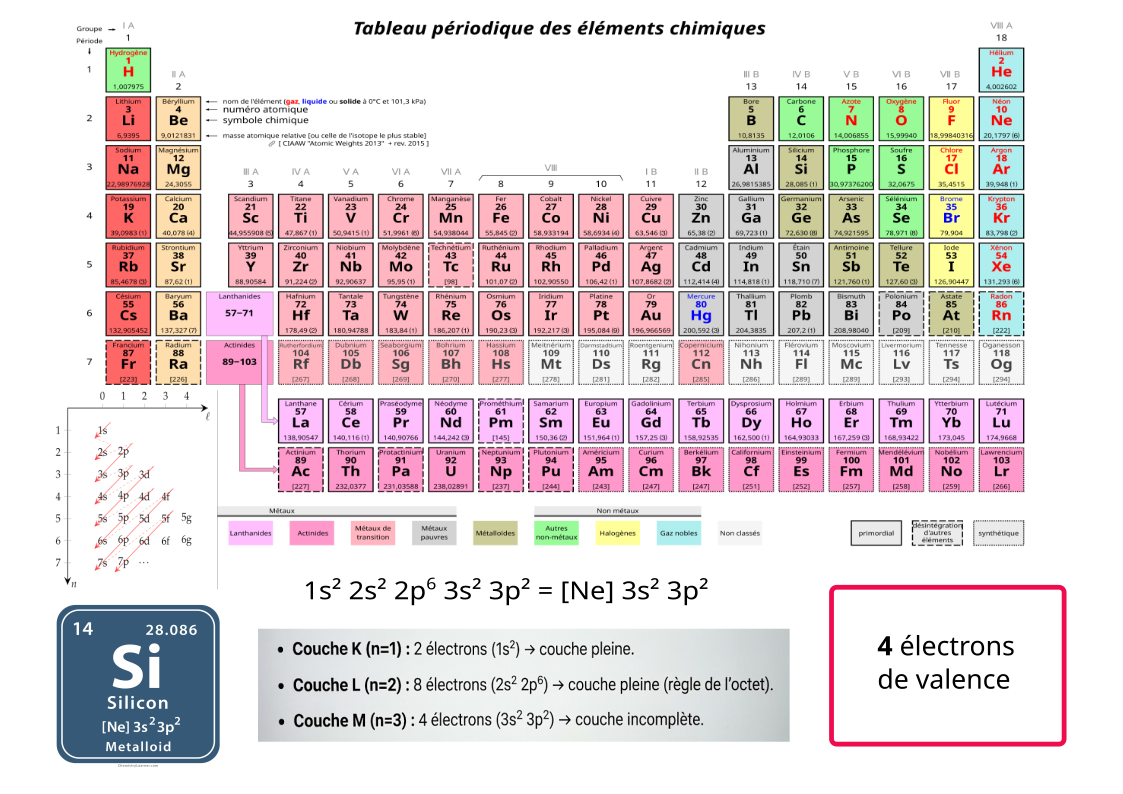
\includegraphics[scale=0.35]{images/silicium_atome.png}
  \end{center}
\end{frame}

\begin{frame}{Le Silicium : à partir de la Silice}
 \begin{enumerate}

   \item \textbf{Extraction} : réduction carbothermique de la silice
   \begin{itemize}
     \item Réaction chimique à 3000° : SiO2 + 2C → Si (liquide) + 2CO (gaz)
     \item Source de carbone : charbon, coke,...
     \item Pureté 98-99.5 \% insuffisante pour l'Electronique (silicium métallurgique MG-Si)
   \end{itemize}

   \item \textbf{Purification} : Procédé \textbf{Siemens}
   \begin{itemize}
     \item Hydrochloration du silicium métallurgique : trichlorosilane $SiHCl_3$ (gazeux)
     \item Si + 3 HCl → SiHCl3 + H2
     \item Distillation : chauffage à 1100°. Décomposition et obtention de "germes".
     \item Pureté 99.9999999\% (polycristallin) voire plus pour l'Electronique.
   \end{itemize}

   \item \textbf{Obtention d'un monocristal} : Procédé \textbf{Czokralski}
   \begin{itemize}
     \item Fusion et germination.
     \item Tirage et rotation.
     \item Formation du lingot.
   \end{itemize}

 \end{enumerate}
\end{frame}

\begin{frame}{Le Silicium : méthode Czokralski}
  \begin{center}
    \includesvg[scale=0.4]{images/silicium_czokralski}
  \end{center}
\end{frame}
